\definecolor{exxetagray}{gray}{0.75}
\definecolor{itemcolor}{RGB}{179,217,255}
\definecolor{usercolor}{RGB}{255,204,179}

\shorthandoff{"}
\chapter{Empfehlungssysteme}
\label{ch:empfehlungssysteme}

\section{Einführung}
\label{ch:empfehlungssysteme:einführung}
Im einfachsten Sinne können Empfehlungssysteme (engl.: \ac{RS}) als Techniken und Werkzeuge verstanden werden, die Nutzern eines Systems aus einer Menge an Elementen potenziell nützliche Elemente vorschlagen \cite[S. 10]{ricci:book}.
% Wie sage ich im einfachsten sinn, wenn es nicht genau so im zitat steht?
Etwas feingranularer definiert \textcite[S. 1]{klahold:book} Empfehlungssysteme als Systeme, die einem Nutzer oder einer Gruppe an Nutzern in einem gegebenen Kontext aus einer Menge möglicher Entitäten eine Teilmenge "nützlicher" Elemente empfehlen.
Aus der Definition von \textcite[S. 1]{klahold:book} lassen sich die grundlegenden Komponenten, die für das Erstellen von Empfehlungen in Empfehlungssystemen von Bedeutung sind, deutlich abgrenzen.
% Andere Wortwahl als "sehr deutlich hervorgehen", will sowas sagen wie, es ist sehr klar zu erkennen, welche komponenten beteiligt sind.
Für ein fundiertes Verständnis sind die einzelnen Komponenten und deren Zusammenspiel in Abbildung \ref{fig:empfehlungssysteme:einführung:abb1} vereinfacht dargestellt.

\begin{figure}[H]
    \centering
	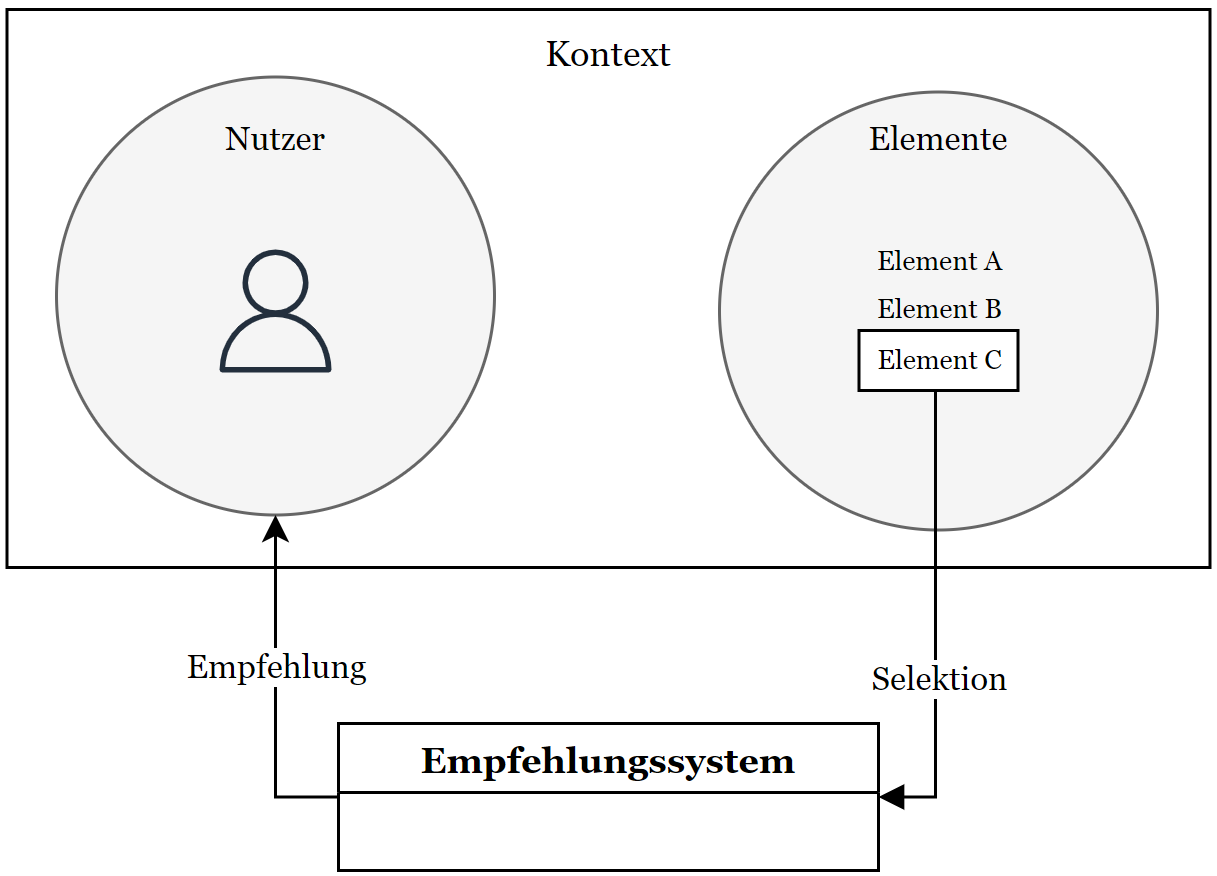
\includegraphics[width=0.8\textwidth]{gfx/komponenten-empfehlungssystem.png}
	\caption[Komponenten eines Empfehlungssystems]{Komponenten eines Empfehlungssystems\\
	(Eigene Darstellung in Anlehnung an \cite[S. 2]{klahold:book})}
	\label{fig:empfehlungssysteme:einführung:abb1}
\end{figure}

Wie aus Abbildung \ref{fig:empfehlungssysteme:einführung:abb1} hervorgeht, stehen sich in  Empfehlungssystemen grundsätzlich zwei Akteure gegenüber.
% Frage: kann man Elemente als "Akteur" bezeichnen oder anderes Wort dafür?
Auf der einen Seite stehen Empfänger von Empfehlungen, welche in Empfehlungssystemen meist als Nutzer bezeichnet werden \cite[S. 8]{ricci:book}.
Dem gegenüber stehen Entitäten, die Nutzern empfohlen werden können.
Entitäten werden in Empfehlungssystemen als Elemente bezeichnet und bilden den Inhalt von Empfehlungen.
Dabei kann es sich bei Elementen sowohl um Gegenstände wie CDs, Bücher und Klamotten handeln, als auch beispielsweise Personen, Orte oder Prozesse.
% Unter dem Kontext einer Empfehlung versteht \textcite[S. 1]{klahold:book} das Zusammenspiel aus der Situation, in der eine Empfehlung gegeben wird, dem Profil eines Nutzers sowie der Menge möglicher Entitäten zum Zeitpunkt einer Empfehlung.
Unter dem Kontext einer Empfehlung verstehen \textcite[S. 191]{ricci:book} zusätzliche Parameter wie Uhrzeit, Ort oder die Gegenwart anderer Personen zum Zeitpunkt einer Empfehlung.\footnote{\textcite[S. 1]{klahold:book} versteht unter dem Kontext das Zusammenspiel aus der Situation, in der eine Empfehlung gegeben wird, dem Profil eines Nutzers sowie der Menge möglicher Entitäten zum Zeitpunkt einer Empfehlung. Es wird angenommen, dass der Kontext nach dem Verständnis von \textcite{ricci:book} gleichzusetzen ist mit der Situation nach dem Verstängnis von \textcite{klahold:book} und die Berücksichtigung von Nutzerprofil und Elementen nach dem Verständnis von \textcite{ricci:book} implizit stattfindet.}

Darüber hinaus können Nutzer in Empfehlungssystemen mit Elementen in Beziehung gesetzt werden.
Beispielsweise kann eine Beziehung zwischen einem Nutzer und einem Element unterstellt werden, wenn ein Nutzer in der Vergangenheit ein Element gekauft oder bewertet hat.
Solche Beziehungen zwischen Elementen und Nutzern in Empfehlungssystemen werden als Nutzer- Element- Interaktion oder Transaktion bezeichnet \cite[S. 8]{recommenderSystems:2016}\cite[S. 9]{ricci:book}.

Neben Transaktionen können Nutzer bzw. Elemente in Empfehlungssystemen zusätzliche Attribute besitzen.
Bekannte Beispiele für Attribute eines Nutzers sind das Geschlecht oder Alter eines Nutzers, während Attribute eines Produktes beispielsweise die Produktkategorie oder der Preis sein können.
% Unterschied Kombination und Interaktion? Kombibnation ist nicht zwangsläufig das vorhandensein einer Interaktion

% Einigung: Nützlichkeit bezieht sich nicht auf die Güte einer Empfehlung, sondern auf den Nutzen einer Kombination. Güte beschreibt Wert einer Empfehlung.
Der Begriff der "Nützlichkeit" wird in der Literatur vermehrt verwendet, um den Wert eines Elements für einen Nutzer zu beschreiben \cite[S. 10f]{ricci:book}\cite[S. 1]{klahold:book}\cite[S. 735]{adomavicius:inproceedings}.\footnote{Unter der Nützlichkeit kann in dem Kontext von Empfehlungssystemen auch die Güte einer Empfehlung verstanden werden \cite[S. 37ff]{klahold:book}.}
Dabei kann der Nutzen sowohl unmittelbar über Angaben eines Nutzers erschlossen, als auch über eine Nutzenfunktion des Empfehlungssystems berechnet werden \cite[S. 735]{adomavicius:inproceedings}.
Da die Ermittlung des Nutzen durchaus komplex sein kann, wird der Aspekt der "Nützlichkeit" in Kapitel \ref{ch:empfehlungssysteme:nutzenfunktion} ausführlich aufgegriffen.

\section{Problemstellung}
\label{ch:empfehlungssysteme:problemstellung}
% Im vorangegangenen Kapitel wurden grundlegende Komponenten von Empfehlungssystemen und deren Zusammenspiel erläutert.
Das grundlegende Problem, welches Empfehlungssysteme zu lösen versuchen, besteht darin, aus einer Menge an Elementen das Element bzw. die Elemente zu ermitteln, von denen angenommen werden kann, dass diese für die Empfänger einer Empfehlung von Relevanz sind \cite[S. 734f]{adomavicius:inproceedings}\cite[S. 76]{jannach:inproceedings}.
Relevanz bedeutet in dem Kontext von Empfehlungssystemen, dass die Empfehlung an einen Nutzer bzw. eine Gruppe an Nutzern einen maximalen Nutzen bietet \cite[S. 49]{adomavicius:inproceedings:2}\cite[S. 219]{lakiotaki:inproceedings}.
Formal ausgedrückt besteht das Problem darin, einem Nutzer $c$ eine Menge an Elementen $s^{'}$ $\in$ $S$ zur Verfügung zu stellen, für die gilt:
\begin{equation}\label{eq1}
    \forall c\in C,  s'_c = arg\max_{s \in S} u(c,s)
\end{equation}
Hierbei gibt $C$ die Menge aller Nutzer eines Systems und $u(c,s)$ den Nutzen einer Kombination an Element s und Nutzer c (im Folgenden Nutzer- Element- Kombination genannt) an \cite[S. 734f]{adomavicius:inproceedings}\cite[S. 219]{lakiotaki:inproceedings}.
Der Kontext $K$ wird in \textcite[S. 1]{klahold:book} explizit für die Ermittlung des Nutzen einer Nutzer- Element- Kombination angeführt.
Grundsätzlich stellen kontextbasierte Empfehlungssysteme, das heißt Syteme, die den Kontext von Empfehlungen für die Ermittlung des Nutzen berücksichtigen, eine Erweiterung traditioneller Empfehlungssyteme dar \cite[S. 744ff]{adomavicius:inproceedings}.
In der Literatur wird der Nutzen einer Nutzer- Element- Kombination traditionell ohne Berücksichtigung des Kontextes betrachtet, weshalb der Kontext von Empfehlungen in dieser Arbeit vernachlässigt wird \cite[S. 734f]{adomavicius:inproceedings}\cite[S. 219]{lakiotaki:inproceedings}\cite[S. 3]{jawaheer:article}.
In Anlehnung an \textcite[S. 3]{jawaheer:article} wird der interessierte Leser für eine detaillierte Übersicht zu kontextbasierten Empfehlungsssystemen auf \textcite[S. 191ff]{ricci:book} verwiesen.
% In den Formulierungen der Gleichung in \cite[S. 734f]{adomavicius:inproceedings} und \cite[S. 219]{lakiotaki:inproceedings} wird jedoch nicht explizit auf den Kontext als Bedingung zur Erfüllung von Gleichung \ref{eq1} hingewiesen.
% Es wird angenommen, dass der Kontext für die Ermittlung der Güte einer Empfehlung implizit berücksichtigt wird und daher auf eine explizite Nennung verzichtet wurde. In Anlehnung an \cite[S. 734f]{adomavicius:inproceedings} und \cite[S. 219]{lakiotaki:inproceedings} wurde daher auf die explizite Unterscheidung im weiteren Verlauf verzichtet.

Da es sich bei dem Problem des Ermittelns einer nutzenmaximierenden Teilmenge aus einer Menge an Elementen um ein Maximierungs- Problem handelt, kann das Problem der Kategorie der Optimierungsprobleme, wie in \textcite[S. 1]{book:kallrath} definiert, zugeordnet werden.

\section{Nutzenfunktion} % Unterschied Nutzen und Güte?
\label{ch:empfehlungssysteme:nutzenfunktion}
% Frage: ist mit der Güte die Güte einer Empfehlung gemeint (gefällt einem nutzer die Empfehlung ja/nein), oder ist damit die Güte im Sinne von die Qualität von Empfehlungssystemen gemeint?
% Der erfolgreiche Einsatz von Empfehlungssystemen wird maßgeblich von der Qualität der ausgesprochenen Empfehlungen bestimmt.
In Kapitel \ref{ch:empfehlungssysteme:einführung} wurde bereits darauf hingewiesen, dass die Ermittlung der "Nützlichkeit" in Empfehlungssystemen durchaus komplex sein kann.

Wie aus Gleichung \ref{eq1} hervorgeht, wird für den Nutzen einer Nutzer- Element- Kombination in Empfehlungssystemen allgemein eine Funktion $u(c,s)$ angenommen.
Diese Funktion wird Nutzenfunktion (engl.: utility function) genannt und ist traditionell definiert als \cite[S. 195]{ricci:book}\cite[S. 3]{jawaheer:article}:
\begin{equation}\label{eq2}
    u: Nutzer \times Element \rightarrow R
\end{equation}
Über die Nutzenfunktion kann für jede Kombination an Nutzer $c \in C$ und Element $s \in S$ eines Empfehlungssystems dessen Nutzen $u(c,s)$ bestimmt werden.
Für alle Kombinationen von $C$ und $S$ eines Empfehlungssystems können die zugehörigen Nutzenwerte in einer $C \times S$ - Matrix abgebildet werden.
Diese Matrix wird auch als Rating-Matrix $R$ bezeichnet \cite[S. 11]{recommenderSystems:2016}\cite[S. 91]{ekstrand:article}.
% Hierbei stellt die Matrix $R$ für jede Nutzer- Element- Kombination deren Nutzen dar \cite[S. 874]{ricci:book}\cite[S. 49]{adomavicius:inproceedings:2}.
% Was genau ist jetzt R0? Matrix oder Wertebereich (Skala)?
% In Systemen, in denen der Wert einer Transaktion beispielsweise über eine explizite, binäre Bewertung (z.B. "Gut", "Schlecht") eines Nutzers für ein Element bestimmt wird, würde $R_{0}$ genau die zwei Ausprägungen umfassen, die eine Bewertung annehmen kann (hier: "Gut" und "Schlecht").

Grundsätzlich kann die Nutzenfunktion in Empfehlungssystemen jede beliebige Funktion darstellen \cite[S. 735]{adomavicius:inproceedings}.
Angenommen das Ziel eines Empfehlungssystems besteht darin, den Gesamtumsatz eines Unternehmens zu maximieren, so kann der Nutzen einer Nutzer- Element- Kombination über eine Profit-Funktion ermittelt werden.
Solche Systeme, in denen der Nutzen von Nutzer- Element- Kombinationen über eine eigenständige Nutzenfunktion ermittelt wird, zählen zu den nutzenbasierten Empfehlungssystemen und sind nicht Inhalt dieser Arbeit.

In den meisten Empfehlungssystemen wird für den Nutzen einer Nutzer- Element- Kombination $u(c,s)$ unmittelbar die Bewertung (engl.: Rating) $r_{cs}$ eines Element $s$ durch einen Nutzer $c$ angenommen \cite[S. 735]{adomavicius:inproceedings}\cite[S. 9]{ricci:book}\cite[S. 11]{recommenderSystems:2016}.
Daher ist die Nutzenfunktion in der Literatur auch als Rating-Funktion bekannt \cite[S. 49]{adomavicius:inproceedings:2}.
% Für den weiteren Verlauf der Arbeit werden daher die Begrifffe Nutzen und Bewertung bzw. Rating synonym verwendet.
% Es wird davon ausgegangen, dass die gängige Verwendung des Ratings als Maß des Nutzen eines Elements für einen Nutzer daher kommt, dass Empfehlungssysteme traditionell in dem Kontext item-to-people-recommendation eingesetzt wurden.
% In solchen systemen ist es meistens das ziel, die elemente zu empfehlen, die den nutzer am meisten ansprechen. -> Folglich Nutzen einer Nutzer-Element-Kombination bedeutet Nutzen eines Elements für einen Nutzer. (kann aber ja auch bedeuten nutzen eines elements für einen nutzer im sinne von profitmaximierung)
% Unter der Annahme ist damit erklärbar, dass mit einer gewissen Konfidenz davon ausgegangen werden kann, dass die Bewertung eines Nutzers für ein Element auch dessen gefühlten Nutzen des ELements für ihn abbildet.

Bewertungen von Elementen in Empfehlungssystemen können sowohl explizit als auch implizit erfolgen.
Unter expliziter Bewertung kann in Empfehlungssystemen die ausdrückliche Bewertung eines Elements durch einen Nutzer verstanden werden.
Ein Beispiel stellt die aktive Bewertung eines Produktes durch einen Nutzer in einem Online-Shop in Form einer Produktrezension (z.B. "Gefällt-mir"-Angabe) dar.
Im Vergleich dazu werden unter impliziten Bewertungen in Empfehlungssystemen passiv erzeugte Verhaltensdaten, wie der Suchverlauf oder die Kaufhistorie eines Nutzers, verstanden, die indirekt mögliche Präferenzen eines Nutzers vermuten lassen \cite[S. 149]{jadidinejad:inproceedings}\cite[S. 403]{unternährer:article}.
% IDEE: hier einfügen Rating Scales? Ordinal, numeric, etc.

Tabelle \ref{tab1} stellt beispielhaft den Ausschnitt einer Rating-Matrix $R$ dar, welche explizite Bewertungen von Mitarbeitern zu ihren Fähigkeiten abbildet \cite[S. 735]{adomavicius:inproceedings}\cite[S. 16]{link:booklet}.
Hierbei stellen Mitarbeiter die Nutzer und Fähigkeiten die Elemente des Systems dar.
Der Nutzen einer Kombination $u(c,s)$ wird unmittelbar über die Bewertung $r_{cs}$ eines Mitarbeiters $c$ für eine Fähigkeit $s$ bestimmt.
% Eine Bewertung kann jeden Wert in $R_{0}=\{1;2;3;4;5\}$ annehmen.

\begin{table}[htbp]
    \begin{center}
    \begin{tabular}{c|c|c|c|c|c|c}
    {} & {\textbf{Java}} & {\textbf{Python}} & {\textbf{MySQL}} & {\textbf{MongoDB}} & {\textbf{HDFS}} & {\textbf{Spark}}\\
    \hline
    \textbf{D., Jane} & ? & 4 & 3 & 3 & ? & ?\\
    \hline
    \textbf{D., John} & 3 & ? & 2 & ? & 1 & ?\\
    \hline
    \textbf{M., Erika} & ? & ? & ? & 3 & 5 & 3\\
    \hline
    \textbf{M., Max} & 2 & 3 & 1 & ? & ? & ?\\
    \end{tabular}
    \end{center}
	\caption{Beispielhafte Darstellung einer Rating-Matrix (in Anlehnung an \cite{link:booklet})}
	\label{tab1}
\end{table}

Der Rating-Matrix $R$ können alle angegebenen Bewertungen von Mitarbeitern zu ihren Fähigkeiten entnommen werden.
So wird beispielsweise ersichtlich, dass Jane D. im Verhältnis zu den anderen Mitarbeitern ihre Fähigkeiten in Python am höchsten bewertet hat.
Darüber hinaus geht aus Tabelle \ref{tab1} hervor, dass einige Nutzer- Element- Kombinationen $r_{cs}$ anstelle einer Bewertung ein Fragezeichen beinhalten.
Das Fragezeichen kennzeichnet die Kombinationen des Empfehlungssystems, für deren Transaktion kein Wert bekannt ist.
Das kann beispielsweise bei Nutzern der Fall sein, die noch keine Elemente bewertet haben, oder bei Elementen, die neu einem System hinzugefügt wurden und noch keine Interaktion mit Nutzern des Systems aufweisen.
Wie im nachfolgenden Kapitel deutlich werden wird, stellt die Vorhersage von Nutzer- Element- Kombinationen für fehlende Transaktionen eine der Kernaufgaben von Empfehlungssystemen dar.
% Zu den Herausforderungen von Empfehlungssystemen zählt das Ermitteln der angenommenen Werte $R(c_{i},s_{j})$ für Nutzer bzw. Elemente, für die keine Bewertungen vorliegen.
% Nach \textcite[S. 37]{klahold:book} besteht eine der Herausforderungen in der Ermittlung des tatsächlichen Nutzen einer Empfehlung darin, dass für eine objektive Beurteilung die genaue Nutzenfunktion einer Empfehlung an einen Nutzer bekannt sein muss.
% In der Praxis gestaltet sich die Bestimmung einer akkuraten Nutzenfunktion zur Ermittlung der Güte einer Empfehlung für die Nutzer eines Systems jedoch zumeist schwierig.
% Hier ergänzen nach gespräch mit Andreas. Quellen dazu: Klahod S. 37ff und hier: https://api-depositonce.tu-berlin.de/server/api/core/bitstreams/b490302e-8b6a-4300-946f-b5763c2b47d7/content
% The design of effective utility functions often requires domain-specific knowledge, or learning data from past user interactions. % aggarwal, S. 178

\section{Erstellen von Empfehlungen}
\label{ch:empfehlungssysteme:empfehlungserstellung}
Das Erstellen von Empfehlungen ist eine nicht-triviale Aufgabe, die bereits seit Jahrzehnten Inhalt zahlreicher Veröffentlichungen und Konferenzen ist.
Grundsätzlich kann das Erstellen von Empfehlungen in Empfehlungssystemen in zwei Phasen unterteilt werden \cite[S. 405]{unternährer:article}\cite[S. 854]{ricci:book}:
\begin{enumerate}
	\item Vorhersage-Phase
	\item Ranking-Phase
\end{enumerate}

In der Vorhersage-Phase wird der Nutzen von Nutzer- Element- Kombinationen vorhergesagt, für die keine Transaktionen vorliegen.
Für die Ranking-Phase werden die (angenommenen) Nutzer- Element- Kombinationen aus Phase 1 herangezogen, in Abhängigkeit ihrer Nützlichkeit sortiert und das Element bzw. die Elemente mit dem größten Nutzen empfohlen.
Nachfolgend werden die einzelnen Phasen im Detail erläutert.

\subsection{Vorhersage}
\label{ch:empfehlungssysteme:empfehlungserstellung:prediction}
% Ratings normalerweise nur vorhanden bei nutzern, die diese produkte in der vergangenheit bewertet haben, S. 735, file://wsl%24/Ubuntu/home/masc6/Projects/masterarbeit/literatur/Toward_the_next_generation_of_recommender_systems_a_survey_of_the_state-of-the-art_and_possible_extensions.pdf
Wie aus Gleichung \ref{eq1} hervorgeht, ist das Vorhandensein eines Wertes für eine Nutzer- Element- Interaktion Voraussetzung, um die Nützlichkeit der Kombination im Vergleich zu anderen Nutzer- Element- Kombinationen zu bewerten.
Eine gängige Eigenschaft von Umgebungen, in denen Empfehlungssysteme ihren Einsatz finden, ist, dass die zugrundeliegenden Daten unvollständig sind \cite[S. 735]{adomavicius:inproceedings}.
Das bedeutet, dass nicht für jede Kombination an Nutzer und Element ein Wert für $r_{cs}$ vorliegt (wie in Tabelle \ref{tab1} durch Fragezeichen gekennzeichnet).
So ist es beispielsweise anhand der Daten aus Tabelle \ref{tab1} nicht möglich zu Beurteilen, welche der beiden Mitarbeiter Jane D. und Erika M. die Fähigkeit Java besser beherrscht.
% Würde beispielsweise für Erika M. aus Tabelle \ref{tab1} versucht zu Bestimmen, ob ihre Fähigkeiten in Java oder Python höher sind, könnte anhand von Gleichung \ref{eq1} aufgrund der fehlenden Nutzer-Element-Interaktion keine Aussage getroffen werden.

Aufgabe eines Empfehlungssystems ist es daher die fehlenden Nutzer- Element- Kombinationen der Rating-Matrix $R$ vorherzusagen.
Für die Vorhersage einer Nutzer- Element- Kombination $\hat{r}_{c,s}$ der Matrix $R$ kann allgemein folgende Formel angenommen werden (in Anlehnung an \cite[S. 743]{adomavicius:inproceedings}):\footnote{Voraussetzung der Gültigkeit der Formel \ref{eq3} ist die Annahme, dass gilt $r_{cs} = u(c,s)$. Das bedeutet, dass für den Nutzen einer Nutzer- Element- Kombination unmittelbar der Wert der Bewertung $r_{cs}$ eines Nutzers $c$ für das Element $s$ angenommen werden kann (Vgl. Kapitel \ref{ch:empfehlungssysteme:nutzenfunktion}).}
\begin{equation}\label{eq3}
\hat{r}_{cs} =
    \begin{cases}
        r_{cs} & \textnormal{wenn } r_{cs} \neq \textnormal{ ?} \\
        u(c,s) & \textnormal{wenn }r_{cs} = \textnormal{ ?} \\
    \end{cases}
\end{equation}
Demnach kann der Wert einer Bewertung $\hat{r}_{c,s}$ vorhergesagt werden, entweder unmittelbar über vorhandene Nutzer- Element- Interaktionen $r_{cs}$, oder unter Anwendung der Nutzenfunktion $u(c,s)$ bei fehlenden Nutzer- Element- Kombinationen.
% Unterschied ist, dass hier rij sich von u unterscheidet und bei uns einfach erstmal R als ein wert angenommen wird
% Wichtig hier klar zu definieren, dass die Nützlichkeit oft so definiert ist, dass sie entweder explizit gegeben ist, oder über u berechnet wird für fehlende werte von r
% bei uns wird dann quasi u für alle werte berechnet, da wir ja nicht explizit einen wert annehmen, sondern Ro sich aus r1 und r2 usw zusammensetzt

In der Praxis existieren verschiedene Techniken, um fehlende Nutzer-Elemet-Kombinationen vorherzusagen.
Empfehlungssysteme können anhand der eingesetzten Technik für die Vorhersage in verschiedene Kategorien unterteilt werden \cite[S. 8 ff]{recommenderSystems:2016}.
Zu den bekanntesten Kategorien von Empfehlungssystemen zählen:
\begin{itemize}%Sind die mathematischen Bezeichnungen hier verwirrend oder sinnvoll?
	\item \textit{Systeme des Kollaborativen Filterns:} Vorhersage fehlender Nutzer- Element- Kombinationen $r_{cs}$ eines Zielnutzers $c$ anhand vorhandener Nutzer- Element- Interaktionen $r_{c's}$ anderer Nutzer $c' \in C \backslash \{c\}$ des Systems, die dem Zielnutzer $c$ ähnlich sind.
	\item \textit{Inhaltsbasierte Systeme:} Vorhersage fehlender Nutzer- Element- Kombinationen $r_{cs}$ eines Zielnutzers $c$ anhand vorhandener Nutzer- Element- Interaktionen $r_{cs'}$ des Zielnutzers zu Elementen $s' \in S \backslash \{s\}$, die dem Zielelement $s$ ähnlich sind.
	\item \textit{Wissensbasierte Systeme:} Vorhersage fehlender Nutzer- Element- Kombinationen eines Zielnutzers anhand der aktiven Angabe von Präferenzen durch den Zielnutzer.
	\item \textit{Hybride Systeme:} Kombination verschiedener Techniken für die Vorhersage fehlender Nutzer- Element- Kombinationen.
\end{itemize}

Der Fokus dieser Arbeit liegt auf der zweiten Phase des Empfehlungserstellungs-Prozesses, weshalb auf eine Erläuterung der Techniken nachfolgend verzichtet wird.
Für eine detaillierte Übersicht der bekanntesten Werkzeuge wird der interessierte Leser auf \textcite[S. 8ff]{recommenderSystems:2016} verwiesen.

\subsection{Ranking}
\label{ch:empfehlungssysteme:empfehlungserstellung:recommendation}
Die zweite Phase umfasst die eigentliche Erstellung der Empfehlungen, die an einen Nutzer zurückgegeben werden.
Das Ziel der zweiten Phase ist es, einem Nutzer $c$ in Abhängigkeit der gegebenen Rating-Matrix $R$ eine Empfehlung an Elementen $s'$ mit dem größtmöglichen Nutzen zu generieren \cite[S. 6]{ekstrand:article}.

In Abhängigkeit des Anwendungsfalls kann eine Empfehlung verschiedene Formen annehmen.
So kann eine Empfehlung eine Gruppe an Elementen darstellen.
Ein Beispiel stellen Empfehlungen auf Webseiten von Klamottenlabeln dar, die verschiedene Kleidungsstücke gemeinsam als vollständige Outfits empfehlen.
In den meisten Fällen geben Empfehlungssysteme eine sortierte Liste der nützlichsten Elemente zurück (Top-K-Elemente), in der für jedes Element der angenommene Wert für einen Nutzer angegeben ist \cite[S. 6]{ricci:book}\cite[S. 3]{recommenderSystems:2016}.
Dabei wird die Nützlichkeit einer Kombination, wie in Kapitel \ref{ch:empfehlungssysteme:empfehlungserstellung:prediction} erläutert, zumeist anhand eines Ratings durch einen Nutzer bestimmt, oder über eine Nutzenfunktion in Phase 1 vorhergesagt.
Diese Ratings erfolgen in gängigen Empfehlungssystemen zumeist anhand eines Kriteriums, beispielsweise in Form eines übergreifenden Ratings für ein Element.

In der Praxis kann es vorkommen, dass von einem vorhergesagten Wert einer Nutzer- Element- Kombination nicht unmittelbar auf den tatsächlichen Rang einer Kombination im Ranking geschlossen werden kann, beispielsweise da noch andere Kriterien den Nutzen (und somit den Rang) einer Kombination beeinflussen \cite[S. 405]{unternährer:article}.
Wie in Kapitel \ref{ch:erweiterungen} deutlich werden wird, ist die Bestimmung des Nutzen eines Elements für einen Nutzer anhand eines einzelnen Kriteriums (e.g. dem Rating) nicht immer ausreichend, um dessen Nutzen zuverlässig zu bestimmen \cite[S. 847]{ricci:book}.
% ------- Hier (oder oben?) kurze Zusammenfassung der Begrifflichkeiten (siehe aggarwal, S. xviii, file:///C:/Users/masc6/OneDrive/Persoenliche_Unterlagen/Uni/Masterthesis/Aggarwal2016_Book_RecommenderSystems.pdf)

Abbildung \ref{fig:empfehlungssysteme:recommendation:abb1} illustriert den Prozess der Empfehlungserstellung am Beispiel eines Ausschnitts der Mitarbeiter-Fähigkeiten Matrix aus Tabelle \ref{tab1}.
Das Beispiel stellt den Empfehlungerstellungsprozess für die Mitarbeiterin Erika M. dar.
Dabei soll mithilfe des Empfehlungssystems die Fähigkeit vorschlagen werden, von der angenommen werden kann, dass Erika M. in dieser Fähigkeit die meisten Kenntnisse im Vergleich zu den anderen Fähigkeiten aufweist (e.g. $argmax(\hat{r}_{\textnormal{Erika M., s}})$).
% am die dieser am Gesucht: Element des Mitarbeiters, für das er/sie die höchsten Fähigkeiten aufweist, bspw. weil vorgeschalgen wird in dem Bereich eine Schulung zu geben, oder MA gesucht wird, der experte in einem bestimmten gebiet ist

\begin{figure}[H]
    \centering
	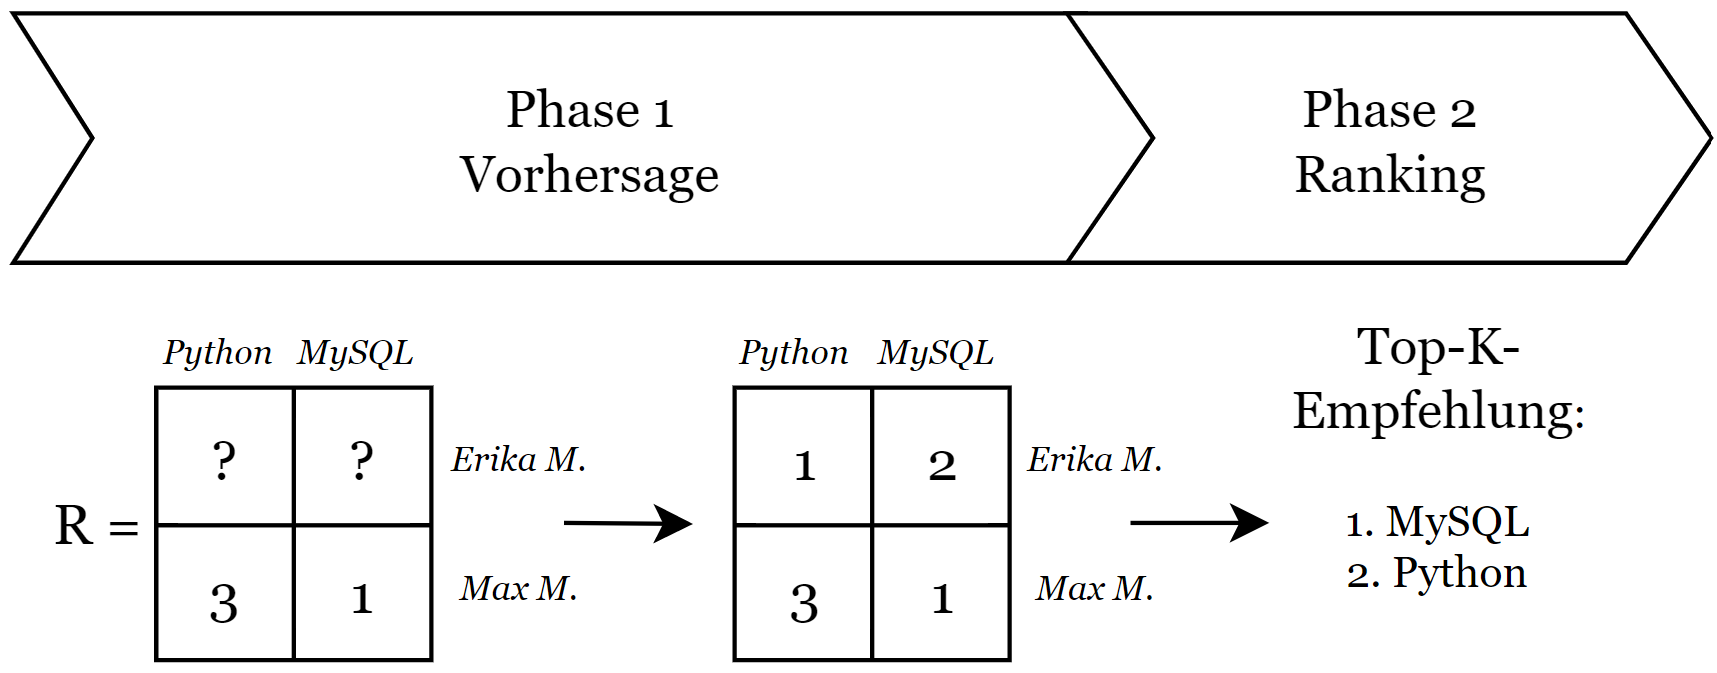
\includegraphics[width=0.9\textwidth]{gfx/phasen-empfehlungserstellung.png}
	\caption[Phasen der Empfehlungserstellung]{Phasen der Empfehlungserstellung\\}
	\label{fig:empfehlungssysteme:recommendation:abb1}
\end{figure}

Empfehlungen dieser Art können beispielsweise sinnvoll sein, wenn Mitarbeitern Fähigkeiten vorgeschlagen werden sollen, die sie verhältnismäßig schnell erwerben können.
% Empfehlungen dieser Art können beispielsweise sinnvoll sein, wenn Mitarbeitern Fähigkeiten vorgeschlagen werden sollen, die viele Ähnlichkeiten zu bereits existierenden Fähigkeiten eines Mitarbeiters aufweisen.
% Dies kann sinnvoll sein, wenn Mitarbeiter möglichst schnell eine Fähigkeit erlernen sollen.
% Wenn angenommen wird, dass Mitarbeiter, die bereits Fähigkeiten besitzen, welche Ähnlichkeiten zu der gefragten Fähigkeit aufweisen, schneller die gefragte Fähigkeit erlernen als Mitarbeiter, die diese Fähigkeiten nicht oder weniger gut beherrschen.
So kann es sinnvoll sein der Mitarbeiterin Erika M. die Fähigkeit MySQL für eine Schulung vorzuschlagen, da aufgrund ihrer Vorkenntnisse in MongoDB angenommen werden kann, dass sie sich MySQL im Verhältnis zu anderen unbekannten Fähigkeiten (z.B. Python) schnell aneignen kann.

\section{Präferenzen in Empfehlungssystemen}
\label{ch:empfehlungssysteme:präferenzen}
Im Zusammenhang mit Empfehlungssystemen fällt häufig der Begriff der Präferenzen (engl.: preferences) \cite[S. 2]{ricci:book}\cite[S. 11f]{recommenderSystems:2016}.
% Brauch man hier überhaupt ein zitat, wenn ich die Annahme selber aufstelle?
In diesem Kapitel werden Präferenzen allgemein erläutert und in dem Kontext von Empfehlungssystemen inhaltlich abgegrenzt.

Nach dem Verständnis der Bundeszentrale für politische Bildung können Präferenzen grundsätzlich als Vorlieben und Verhaltensweisen von Personen verstanden werden, "[...], die bewirken, dass Güter unterscheidbar werden."\cite{pollert:book}
Ein einfaches Beispiel der Präferenzen von Personen stellt die Vorliebe von Schülern für bestimmte Fächer in der Schule dar.
Hierbei sind Schüler die Personen, die Präferenzen besitzen und Güter die verschiedenen Fächer, die Schüler besuchen müssen.
Basierend auf verschiedenen Gründen können Schüler bestimmte Fächer präferieren.
Das heißt, dass sie einige Fächer gegenüber Anderen bevorzugen können.

Wenn Präferenzen in dem Kontext von Empfehlungssystemen aufkommen, wird sich in der Regel auf die Vorlieben und Verhaltensweisen der Nutzer des Systems bezogen.
Beispielsweise kann unter der Präferenz eines Nutzers in einem Online-Shop die Bevorzugung eines Produktes gegenüber eines Anderen Verstanden werden.

Ein Verständnis der Präferenzen von Nutzern eines Systems kann für die erfolgreiche Ermittlung von Empfehlungen von großer Bedeutung sein. % \cite[S. 1]{jawaheer:article}
Für die Ermittlung der Präferenzen von Nutzer in Empfehlungssystemen werden maßgeblich explizite und implizite Bewertungen herangezogen \cite[S. 1]{jawaheer:article}.\footnote{Vgl. Kapitel \ref{ch:empfehlungssysteme:nutzenfunktion}.}
Die Ermittlung der Präferenzen ist jedoch keinesfalls trivial.
Dies hängt unter anderem damit zusammen, dass einer expliziten Bewertung (z.B. einer Gefällt-mir-Angabe in Facebook) durch einen Nutzer aus der Sicht eines Nutzers ein unterschiedlicher Wert zukommen kann als aus Sicht des Systems.
Darüber hinaus kann auch die Bewertungsskala eines Elements Einfluss auf die Genauigkeit von Präferenzen haben.
So kann eine fehlende Gefällt-mir-Angabe für ein Element durch einen Nutzer in Facebook nicht zwangsläufig als Abneigung für das Element verstanden werden \cite[S. 11]{recommenderSystems:2016}.

Anhand von Präferenzen ist es möglich Empfehlungen für Nutzer eines Empfehlungssystems zu personalisieren.
In Abhängigkeit des Grads der Personalisierung können Empfehlungen personalisierten bzw. nicht-personalisierten Empfehlungen zugeordnet werden (in Anlehnung an \cite[S. 400]{unternährer:article}).

\subsection{Personalisierte und Nicht-Personalisierte Empfehlungen}
Unter nicht-personalisierten Empfehlungen versteht \textcite[S. 400]{unternährer:article} Empfehlungen, die allen Nutzern die gleichen Elemente anzeigen.
Das bedeutet, alle Nutzer eines Empfehlungssystems bekommen, unabhängig von deren Präferenzen oder Nutzerprofil, dieselben Elemente vorgeschlagen (z.B. "Top 10 Lieder aller Zeiten").

Für die Ermittlung nicht-personalisierter Empfehlungen können Popularitätsmetriken herangezogen werden.
Dies folgt der Annahme, dass Popularität einen guten Prädiktor der Präferenzen aller Nutzer eines Systems darstellt \cite[S. 406]{unternährer:article}.
Popularitätsmetriken stellen sortierte Listen dar, über die Elemente in ordinale Relationen gesetzt werden können (e.g. Element A ist "besser" als Element B, da es einen höheren Rang aufweist) \cite[S. 404ff]{unternährer:article}.
Die Listen werden basierend auf "aggregierten Präferenzen" aller Nutzer eines Systems generiert.
Hierfür muss im Vorfeld bestimmt werden, welcher Indikator für die Bestimmung der Popularität in einem System geeignet ist (z.B. die Anzahl an Klicks oder Gefällt-mir-Angaben) \cite[S. 406]{unternährer:article}.

Nicht-personalisierte Empfehlungen müssen nicht allein auf absoluter Popularität beruhen.
Nach \textcite[S. 405]{unternährer:article} ermöglichen zeitlich, räumliche und soziale Popularität, absolute Popularität zu begrenzen.
So können Nachrichten-Plattformen beispielsweise gezielt die populärsten Artikel des Tages (zeitliche Popularität) auf ihrer Startseite anzeigen, anstelle der populärsten Artikel aller Zeiten (absolute Popularität).
Unter der Annahme, dass die Relevanz der Beiträge mit deren Aktualität zusammenhängt, kann durch Verwendung von zeitlicher Popularität für die Ermittlung von Empfehlungen die Relevanz von Beiträgen auf der Startseite erhöht werden \cite[S. 405]{unternährer:article}.
% Fragwürdig, ob das nicht auch schon eine art der personalisierung ist? Es ist anzunehmen, dass nicht-personalisiert einfach bedeutet, dass nicht die präfeenzen eines nutzers speziell verwendet werden, um gezielt empfehlungen zu schalten, sondern eben allgemein

Der maßgebende Unterschied zu personalisierten Empfehlungen besteht darin, dass das Erstellen von nicht-personalisierten Empfehlungen für einen Nutzer nicht auf dessen individuellen Präferenzen beruht.
Empfehlungen können somit völlig unabhängig davon erstellt werden, ob ein Nutzer eines Empfehlungssystems bereits eine Interaktion mit einem System aufweist oder nicht.
Dies ermöglicht Systemen auch Empfehlungen für Nutzer zu erstelllen, für die beispielsweise keine Präferenzen bekannt sind.\footnote{Das Problem ist in der Literatur als das Kaltstart-Problem bekannt \cite[S. 407]{unternährer:article}.}
Ausschlaggebend ist lediglich, dass Informationen vorliegen, die es ermöglichen die Popularität von Elementen zu ermitteln.
So kann beispielsweise kein populärster Artikel des Tages einer Nachrichten-Plattform basierend auf der Popularität ermittelt werden, wenn überhaupt keine Interaktionen mit Artikeln des Systems vorliegen.

Im Gegensatz zu nicht-personalisierten Empfehlungen stellen personalisierte Empfehlungen Vorschläge dar, die basierend auf individuellen Präferenzen von Nutzern erstellt werden (bspw. über explizites oder implizites Feedback).
Der Grad der Personalisierung ermöglicht eine weitere Unterteilung der personalisierten Empfehlungen in schwach-personalisierte Empfehlungen und stark-personalisierte Empfehlungen.
Unter schwacher Pesonalisierung versteht \textcite[S. 407]{unternährer:article} stereotypisierende Empfehlungen, die Nutzer, basierend auf deren Attributen (z.B. Wohnort, Alter, Geschlecht), bestimmten Kategorien zuordnen.
Prinzipiell ähneln schwach-personalisierte Empfehlungen den nicht-personalisierten Empfehlungen, da sie auch basierend auf Popularitätsmetriken erstellt werden.
Der Unterschied besteht darin, dass die Popularität von Elementen innerhalb einer Kategorie ermittelt wird.
Die Empfehlungen der populärsten Elemente für einen Nutzer erfolgen dann in Abhängigkeit der kategorialen Zugehörigkeit des Nutzers \cite[S. 407ff]{unternährer:article}.

Stark-personalisierte Empfehlungen verzichten auf pauschale und kategoriale Vorentscheidungen und beziehen sich für das Ermitteln von Empfehlungen auf paarweise Relationen (sog. "Good Matches") zwischen Nutzern untereinander bzw. zwischen Nutzern und deren Elementen \cite[S. 415]{unternährer:article}.
Solche Sachverhalte sind vorwiegend in Systemen des Kollaborativen Filterns und Inhaltsbasierten Empfehlungssystemen anzutreffen.
Hierbei werden nicht einzelne Nutzer oder Elemente bewertet, etwa wie viele Fünf-Sterne-Rezensionen ein Produkt erhalten hat. 
Stattdessen wird der "Fit" einer Kombination an Nutzer und Element bewertet.
Das bedeutet, es wird eine Relation zwischen einem  Nutzer und einem Element erstellt, die dann mit anderen Relationen verglichen werden kann.
Beispielsweise kann eine Fünf-Sterne-Bewertung eines Produktes durch einen Nutzer als starker "Fit" des Produktes mit dem Nutzer gesehen werden.
Diese Beziehung zwischen Nutzer und Produkt kann dann mit anderen Beziehungen verglichen werden, um daraus Präferenzen von Nutzern abzuleiten \cite[S. 417]{unternährer:article}.
% Popularitätsmetriken bewerten, wie gut ein element ist und ob es besser oder schlechter als ein anderes ist, während personalisierte empfehlungen beziehungen zwischen nutzern und elementen bewerten

\subsection{Zugrundeliegende Datenstruktur}
Abhängig von der Art der Empfehlung, liegen in Empfehlungssystemen unterschiedliche Datenstrukturen vor.
% Frage ist, wie Präferenzen denn dargestellt werden, im sinne der Datenstruktur. Also wenn wir von der Matrix oben ausgehen
% Bei popularität: nur bewertung von element ist ausschlaggeben, ggf. noch kategorie, aber sonst reicht bewertung, um ordinale Relation zu erstellen -> d.h. über alle nutzer verteilt die durchschnittlich höchste bewertung -> es existieren nicht wirklich individuelle präferenzen, eher ableitung aus aggregierten präferenzen
% Bei paarweiser Relation: Bewertung einer Beziehung, d.h. betrachten von beziehungen zwischen Nutzern und Elementen, bzw. sogar zwischen Nutzer und Nutzern -> präferenz bedeutet hier die ordinale ordnung von elementen für einen Nutzer (hier habe ich leider keine referenz zu literatur, lediglich eine annahme, muss also weiterschauen)
% das ist der wichtige unterschied zu uns, da wir präferenzen als ein attribut des mitarbeiters bzw als ein attribut des nutzers verstehen, und nicht als interpretation einer relation

% HIER WEITERMACHEN

\section{Wechselseitige Empfehlungssysteme}
\label{ch:empfehlungssysteme:rrs}

\subsection{People-to-People-Empfehlung}
\label{ch:empfehlungssysteme:rrs:people_to_people}

\subsection{Problemstellung}

\shorthandon{"}